\section{Retrieval with MIPS}
In Section \ref{5.6.3} we introduced the notion of \textbf{first stage retrieval}, which is an operation that takes as input the vector representations of documents and queries and produces a ranking of the documents w.r.t. the queries. The main features of this operation are:

\begin{itemize}
    \item it is \textbf{cheap}, since in involves linear function, such as the \textit{inner product}, so it can be implemented for very large collections of documents and queries;
    \item it is \textbf{effective}, i.e. it allows to discard all the non relevant documents, in order to reduce the size of the corpus for the following stages of the cascade.
\end{itemize}

In this section we address the first stage retrieval as a \textbf{MIPS} (or \textbf{Maximum Inner Product Search}) problem, which can be described as follows: given a query vector $q \in \mathbb{R}^n$ and a set of document vectors $D \subset \mathbb{R}^n$, the goal is to find the \textbf{top-$k$ documents} with maximal inner product with $q$, i.e.:

$$
\varsigma = \max_{d \in D}^{(k)} \langle q,d \rangle
$$

In general, the solution of this problem scales well for very large collections since the documents representation $\phi_d$ can be pre-computed, so the only operation that are done at query time are:

\begin{itemize}
    \item representation of the queries $\phi_q$;
    \item computation of the dot product.
\end{itemize}

There exist some algorithms for solving the \textit{MIPS} problem when the queries and the documents are provided as sparse and dense vector, but in general the brute-force approach has a complexity of $O(nm + n\log k)$, where:

\begin{itemize}
    \item $nm$ is given by the dot product;
    \item $n \log k$ is given by the sorting operation of the top-$k$ results, using HeapSort.
\end{itemize}

In Section \ref{sparse} and \ref{dense} we discuss two different methods for representing the queries and the documents, while in Section \ref{mips for sparse} and \ref{mips for dense} we address some algorithms for solving the MIPS problem when the documents and the queries are either sparse or dense.

\subsection{Sparse representation}\label{sparse}
In general, when we're asked to measure the relevance of a document w.r.t. an input query, there exist two main indicator of relevance:

\begin{itemize}
    \item the \textbf{frequency} of a query term in the document;
    \item the \textbf{propensity} of a term in the document, i.e. how much information the term provides to the document. Intuitively, the more common a term is, the less information it conveys.
\end{itemize}

The first indicator is measured by the \textbf{term frequency (TF)}: for a query term $q_t \in q$, the term frequency w.r.t. a given document $d$ is defined as:

$$
TF(q_t, d) = |\{ d_i | q_t = d_i, d_i \in d \}|
$$

, while the second one is measured by the \textbf{inverse document frequency (IDF)}: for a query term $q_t \in q$, the inverse document frequency w.r.t. the collection of documents $D$ is defined as:

$$
IDF(q_t) = \log (1 + \frac{|D| - DF(q_t) + 0.5}{DF(q_t) + 0.5})
$$
, where:

\begin{itemize}
    \item $DF(q_t) = |\{ d | q_t \in d, d \in D \}|$ is the \textbf{collection frequency} of $q_t$, i.e. the number of documents containing the query term $q_t$;
    \item 0.5 is a quantity that ensures that we do not divide by 0.
\end{itemize}

Another possible measure for the frequency of a term is provided by the \textbf{TF$_{\textbf{BM25}}$}, which is define as:

$$
TF_{\text{BM25}}(q_t,d) = \frac{TF(q_t,d)  (k_1 + 1)}{TF(q_t,d) + k_1 (1 - b + b \frac{|D|}{l})}
$$
, where $k_1$ and $b$ are hyperparameters and $l$ is the average lenghts of the documents in the collection. Notice that in this case, $0 \leq TF_{\text{BM25}} \leq 1$.

In this sense, we can compute the impact score of query-document pair in the following sum:

$$
\text{score}(q,d) = \sum_{q_t \in q} TF(q_t,d) \cdot IDF(q_t)
$$

or

$$
\text{score}_{\text{BM25}}(q,d) = \sum_{q_t \in q} TF_{\text{BM25}}(q_t,d) \cdot IDF(q_t)
$$

From a mathematical point of view, the \textit{sparse} score of a document w.r.t. a given query is basically represented by the dot product between the $TF$ (or $TF_{\text{BM25}}$) and the $IDF$ vectors. Let $V$ be a vocabulary, $\Vec{d} \in \mathbb{R}_{+}^{|V|}$ be a vector whose $i$-th coordinate records the importance of the $i$-th term in $V$, i.e. the $TF$ (in the case of BM25, the $TF_{\text{BM25}}$), and $\Vec{q} \in \mathbb{R}_{+}^{|V|}$ be a vector whose $i$-th coordinate records the count of the $i$-th term of $V$ in the query, i.e. the $IDF$, then:

$$
\text{score}(q,d) = \langle \Vec{q}, \Vec{d} \rangle
$$

,or

$$
\text{score}_{\text{BM25}}(q,d) = \langle \Vec{q}, \Vec{d} \rangle
$$

Notice that in this case:

\begin{itemize}
    \item $\Vec{q}$ and $\Vec{d}$ are \textbf{sparse} vectors, i.e. very few coordinates are non-zero in each vector, and every coordinate is non-zero in very few vectors;
    \item $\Vec{q}$ and $\Vec{d}$ are \textbf{non-negative} vectors.
\end{itemize}

\begin{figure}[h!]
		\centering
		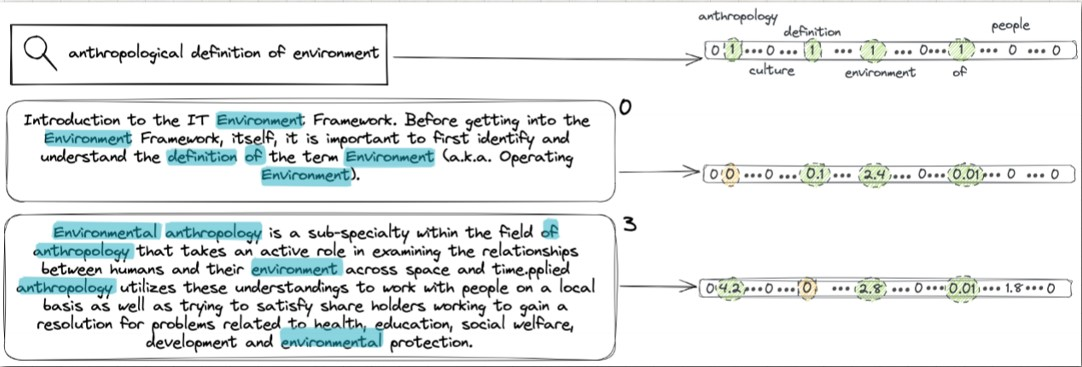
\includegraphics[scale = 1.2]{img/sparse.jpg}
        \label{sparse}
        \caption{Sparse representation of documents w.r.t. an input query}
\end{figure}

\subsubsection{Learning term importance}
We now address the problem of learning the \textit{term frequency}, and in particular we consider the \textbf{Deep Contextualized Term Weighting} (or \textbf{DeepCT}). In this case each term frequency is defined as:

$$
TF(q_t, d) = \begin{cases}
    w(q_t; d), \qquad q_t \in d \\
    0, \qquad \text{otherwise}
\end{cases}
$$
, where $w$ is a regression function that predicts a value given a term in the context of a document. In this case the \textbf{training set} is represented by the collection $D$ of query-document pairs, and the objective is the \textbf{MSE} associated with the following metric:

$$
QTR(t,d) = \frac{|\{ q | (q,d) \in D \land \ t \in d \}|}{|\{ q | (q,d) \in D \}|} 
$$
, i.e. the fraction of queries that contain the term $t$.

Another important concept in ranking is the \textbf{query expansion}, that is represented in Picture \ref{query exp}.

\begin{figure}[h!]
		\centering
		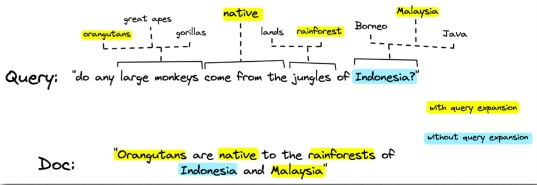
\includegraphics[scale = 1.8]{img/query expansion.jpg}
        \label{query exp}
        \caption{Example of query expansion}
\end{figure}

As we can see, the term overlap between the document and the query without query expansion is represented only by the term \textit{Indonesia} (\textbf{vocabulary mismatch} problem), while exploiting the query expansion method we notice that the document results to be very relevant w.r.t. the query. A famous model for query/document sparse expansion is \textbf{SPLADE}, which exploits the BERT MLM (Masked Language Model) for encouraging sparsity via regularization. The main features of this model are that it produces sparse expansion which are also semantically similar to the original terms of query/document.

Finally, one last important concept is \textbf{query prediction}, i.e. predicting a possible query for an input document. This operation works as follows: the query predictor receives as input a document $d$, and it produces as output the top-$k$ query terms with highest probability. Then, the term with highest probability is sampled, and it is provided as input again to the query predictor: as scheme of the functioning is provided in Picture \ref{query pred}.

\begin{figure}[h!]
		\centering
		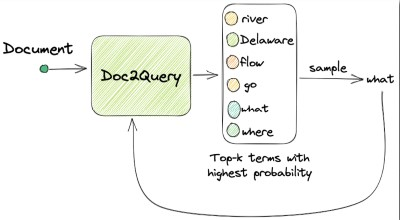
\includegraphics[scale = 1.8]{img/query prediction.jpg}
        \label{query pred}
        \caption{Example of query prediction}
\end{figure}

A famous model for query prediction is \textbf{Doc2Query}, which is characterized by the following advantages:

\begin{itemize}
    \item All the operations are done offline, since the query does not need any type on transformation;
    \item It helps the vocabulary mismatch problem, since it performs an expansion using terms that are not present in the document;
    \item It optimizes log-likelihood: $- \sum_{i = 1}^{|q|} \log P[q_i | q_{<1}, d]$
\end{itemize}

\subsection{Dense representation}\label{dense}
The idea of \textbf{dense representation} is that instead of learning a function $\phi(q,d)$ to represent a query-document pair (Picture \ref{dense 1}), we can separately learn $\phi_q$ and $\phi_d$ to represent query and documents, respectively (Picture \ref{dense 2}). In this way, we can perform the dot product (linear operation) between the two representations, which have a good quality, since the similarity of original queries/documents is preserved in the dense vectors.

\begin{figure}[h!]
		\centering
		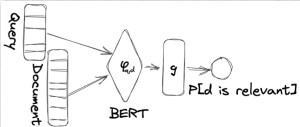
\includegraphics[scale = 1.8]{img/dense 1.jpg}
        \label{dense 1}
        \caption{Original query-document representation}
\end{figure}

\begin{figure}[h!]
		\centering
		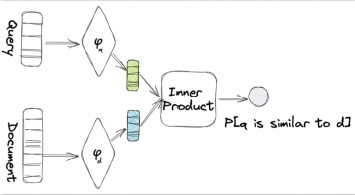
\includegraphics[scale = 1.8]{img/dense 2.jpg}
        \label{dense 2}
        \caption{Dense representation}
\end{figure}

We recall that we introduced \textit{Skip-gram} and \textit{Continuous Bag of Words} for representing \textbf{words} as vectors, but there exist some models for representing \textbf{sentences} as vectors, such as \textbf{Sentence BERT}. This model is trained on pairs of similar sentences: it takes as input two sentences and produces in output the probability that the sentences are similar, as showed in Picture \ref{sentence bert}.

\begin{figure}[h!]
		\centering
		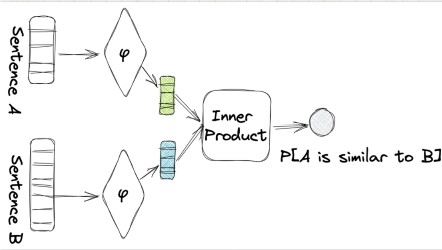
\includegraphics[scale = 1.6]{img/sentence bert.jpg}
        \label{sentence bert}
        \caption{Sentence BERT}
\end{figure}

However, since our goal is to assess the relevance of a (long) document w.r.t. a (short) query, if a term is rare (whether in query or document), its embedding less accurately captures its semantics. That's because the embedding model doesn't see all the term's usage examples and contexts. So its model of the semantics of a rare term in a sentence is more noisy.

Finally, a document can also be split up into several passages, so we can consider a model that represents \textbf{passages} as vectors, such as \textbf{Deep Passage Retrieval (DPR)}. The goal of this model is to learn two different representations $\phi_q$ and $\phi_d$, and it is trained on a dataset composed of a query, a positive document and many negative documents. Then, the model optimizes an inner product ranker's loss to learn better representations $\phi_q$ and $\phi_d$. 

\begin{figure}[h!]
		\centering
		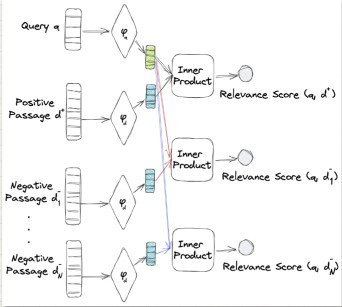
\includegraphics[scale = 2.0]{img/dpr.jpg}
        \label{dpr}
        \caption{Deep Passage Retrieval (DPR)}
\end{figure}

Clearly, the peculiarity of this model is represented by the presence of \textbf{negative documents} in the training set, but where do these negative docs come from? Intuitively, any non-positive example is good, so which one do we pick?

A possible strategy could be the following one:

\begin{enumerate}
    \item Compute the BM25 score between the query and each of the document in the collection;
    \item Select another document randomly form the corpus ($d^{+}$ in the Picture);
    \item Perform in-batch negative sampling among the non-relevant documents, i.e. all the documents $d \neq d^{+}$. Usually, the in-batch negative sampling is performed by providing a batch as input to a model, then propagate the error of the loss function back to the model, in order to change its parameters.
\end{enumerate}

\begin{figure}[h!]
		\centering
		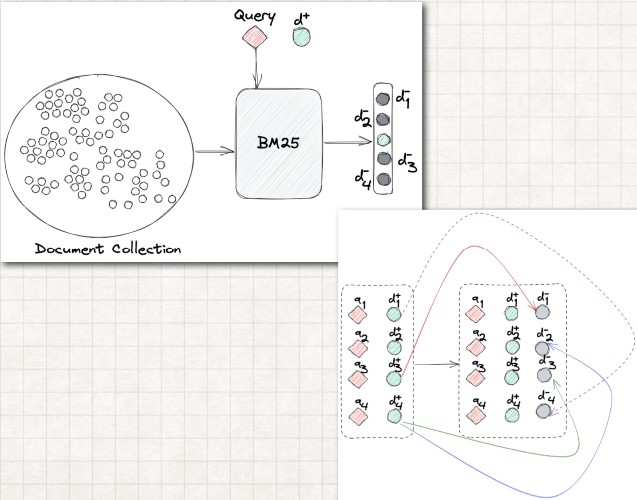
\includegraphics[scale = 1.8]{img/negative sampling 1.jpg}
        \label{negative 1}
        \caption{A possible strategy for negative sampling}
\end{figure}

The \textbf{advantage} of this method is that the non-relevant documents retrieved by \textit{BM25} are syntactically relevant w.r.t. the query, but not semantically, so choosing them as negative examples for the model is very useful for improving its accuracy. However, this method suffers of two \textbf{disadvantages}:

\begin{itemize}
    \item If the queries are very similar, then the documents are very similar too, so the negative examples that are retrieved by the method are not significant;
    \item On the other hand, if the queries are very dissimilar, the negative examples are trivial to be learned.
\end{itemize}


Another possibile method is \textbf{ANCE}, which finds negative examples by retrieving over the current learnt representations, and it works as follows:

\begin{enumerate}
    \item Computes the embedding for each document of the corpus using the representation function $\phi$;
    \item Performs MIPS to retrieve the non-relevant documents;
    \item The non-relevant documents are used for training the representation function $\phi$.
\end{enumerate}

\begin{figure}[h!]
		\centering
		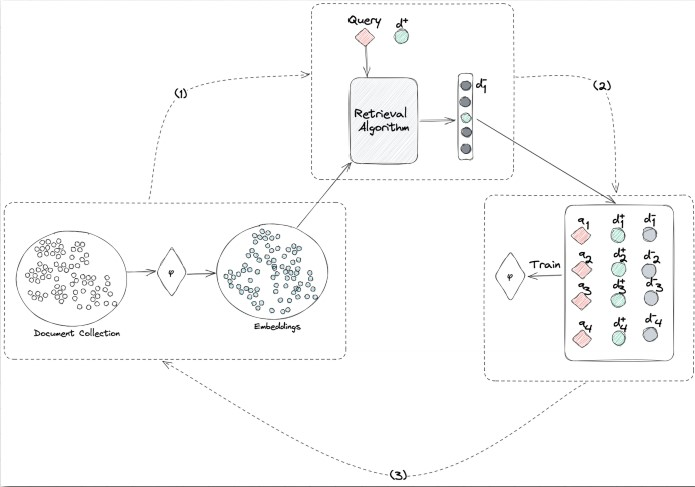
\includegraphics[scale = 1.8]{img/negative sampling 2.jpg}
        \label{negative 2}
        \caption{ANCE method for negative sampling}
\end{figure}

The \textbf{advantage} of this method is that it is quite accurate, but on the other hand it is very expensive, since it asks every time to compute $\phi(d)$, for each $d \in D$, so it suffers of a very slow tuning phase.

Once we discussed the main methods for representing queries and documents, we can now discuss the possible solution for solving the MIPS problem:

$$
\varsigma = \max_{d \in D}^{(k)} \langle \phi(q),\phi(d) \rangle
$$

\subsection{MIPS algorithms for sparse vectors}\label{mips for sparse}
We now discuss some algorithms for solving the MIPS problem when both the documents and the queries are represented as \textbf{sparse vectors}.

The first issue we have to solve is how to represent sparse vectors: one naive representation could be a $|D| \times m$ matrix, as represented in Picture \ref{matrix}.

\begin{figure}[h!]
		\centering
		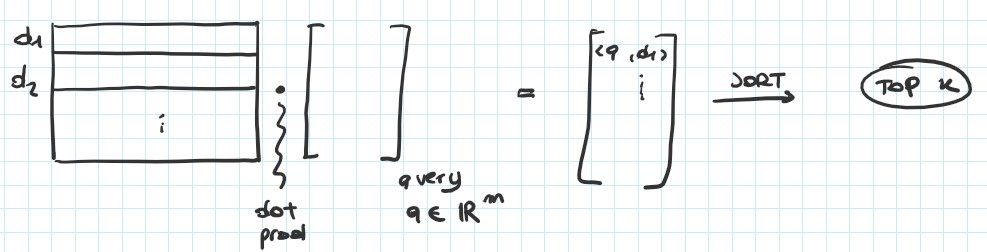
\includegraphics[scale = 1.5]{img/matrix.jpg}
        \label{matrix}
        \caption{Matrix for sparse vectors}
\end{figure}

However, this representation is quite expensive, both in space and time (the sort operation takes $O(|D| \log k)$ time).

In this sense, we can exploit the sparse nature of the vectors by removing all the 0s and represent documents and queries as an \textbf{inverted index}. An inverted index is composed of:

\begin{itemize}
    \item A \textbf{term identifier};
    \item An \textbf{inverted list}, that consists of pairs (docID, score), where the score represents the impact score of the term for that document, for each docID that contains the term. Formally, each entry of the inverted list is $L[i] = \{ (j, d_j[i] | d_j[i] \neq 0) \}$
\end{itemize}

An example of inverted index is provided in Picture \ref{inv ind}.

\begin{figure}[h!]
		\centering
		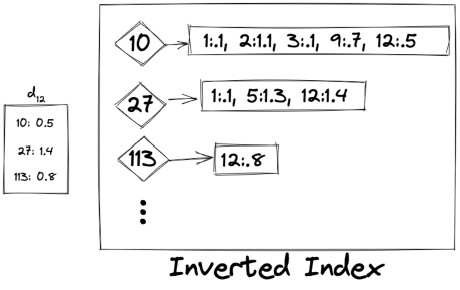
\includegraphics[scale = 1.8]{img/inverted index.jpg}
        \label{inv ind}
        \caption{Example of inverted index}
\end{figure}

Analogously, a query is then represented as a list of terms.

We now discuss two possible methods for query processing, i.e. for retrieving the top-$k$ sparse documents w.r.t. a sparse query.

\subsubsection{TAAT query processing}
The first method we discuss is defined as \textbf{TAAT} query processing, and the idea is that for each term of the query, we build a vector $v \in \mathbb{R}^{|D|}$, s.t. $v[i]$ contains the product between the impact score of the query term and the impact score of document $d_i$. Clearly, if a document does not contain a query term, the corresponding impact score is 0. A visual representation of this method is provided in Picture \ref{taat}.

\begin{figure}[h!]
		\centering
		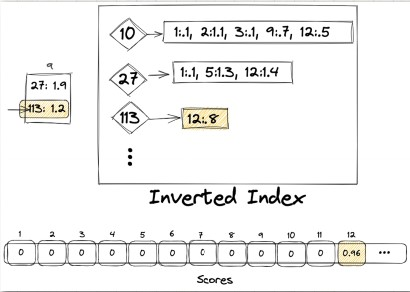
\includegraphics[scale = 1.8]{img/taat.jpg}
        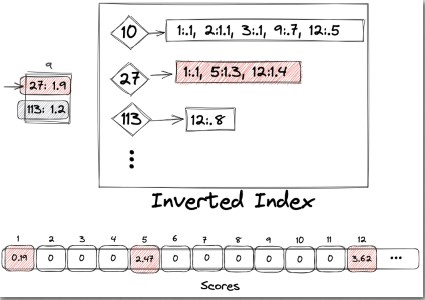
\includegraphics[scale = 1.8]{img/taat 2.jpg}
        \label{taat}
        \caption{Example of TAAT query processing}
\end{figure}

More formally, the algorithm takes as input an inverted index $L$ and a query vector $q$, and it is described in \ref{TAAT}.

\SetKwComment{Comment}{/* }{ */}

\begin{algorithm}[]
\caption{TAAT query processing}\label{TAAT}
\KwData{$L$, $q$}
\KwResult{Top-$k$ document vectors with scores}
$\textit{Scores}[1:|D|] \gets 0$\;
\For{$i$ s.t. $q[i] \neq 0$}{
\For{$(j, d_j[i]) \in L[i]$}{
$\textit{Scores}[j] \gets \textit{Scores}[j] + q[i] d_j[i]$
}
}
Sort $\{ 1, 2, .., |D| \}$ by \textit{Scores}[] in descending order\;
Return top-$k$ identifiers with corresponding scores\;
\end{algorithm}

\subsubsection{DAAT query processing}

\begin{figure}[h!]
		\centering
		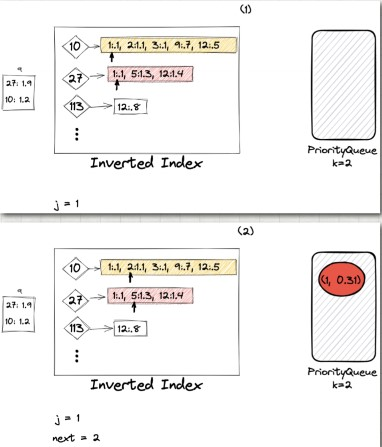
\includegraphics[scale = 1.8]{img/daat.jpg}
        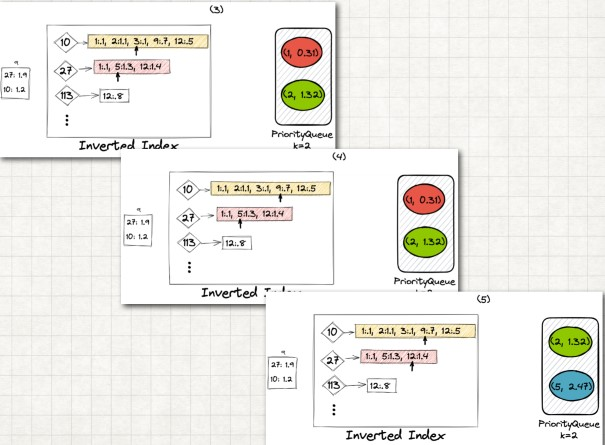
\includegraphics[scale = 1.8]{img/daat 2.jpg}
        \label{daat}
        \caption{Example of DAAT query processing}
\end{figure}

Here the algorithm receives as input an inverted index $L$ where the inverted lists are sorted by docID, and a query vector $q$, and it is described in \ref{DAAT}.

\begin{algorithm}[]
\caption{DAAT query processing}\label{DAAT}
\KwData{$L$, $q$}
\KwResult{Top-$k$ document vectors with scores}
$Q \gets \text{PriorityQueue}$\;
$p[i] \gets 0 \qquad \forall_{i : q_[i] \neq 0}$\;
$j \gets \text{min} \{ j | (j, .) \in L[i], \forall i \}$\;
\While{$p[i] < |L[i]| \qquad \forall i$}{
$\textit{Score} \gets 0$\;
$\text{next} \gets \infty$\;
\For{$i$ s.t. $q[i] \neq 0$}{
\If{$j = L[i][p[i]].\text{id}$}{
$\textit{Score} \gets \textit{Score} + q[i] \times L[i][p[i]].\text{weight}$\;
$p[i] \gets p[i] + 1$
}
\If{$L[i][p[i]] < \text{next}$}{$\text{next} \gets L[i][p[i]].\text{docID}$}
}
$Q$.Push(($j, \textit{Score}$))\;
\If{$|Q| > k$}{$Q$.Pop()}
$j \gets \text{next}$\;
}
Return $Q$\;
\end{algorithm}

\subsubsection{Dynamic pruning algorithms}
Since users are mostly interested in the top few pages of results for a query, the complete scoring of every document that contains at least one query term results in high latency. However, not all of these documents will make the top-$K$ retrieved set of documents that the user will see. Two main general approaches have been exploited to \textbf{increase the efficiency} of \textbf{query processing} in IR systems in the top-$K$ ranked retrieval scenario: 

\begin{enumerate}
    \item Avoid wasting time in processing portions of the inverted index containing documents that are unlikely to be relevant;
    \item Improve the efficiency of algorithms when processing portions of the inverted index containing relevant documents
\end{enumerate}

One of the main design solutions for dealing with these two approaches can be implemented at the query processing level, i.e., by modifying the behaviour of the retrieval algorithms to try to prune documents that will not be retrieved in the top-$K$ . In this section, we summarise the growing literature on dynamic pruning optimisation techniques that improve the query processing efficiency for both the TAAT and DAAT retrieval strategies.

While static pruning strategies alter the index structure at index construction time, \textbf{dynamic pruning} aims to \textbf{alter query processing} in such a way that potentially \textbf{non-relevant documents}, for a given query, \textbf{can be efficiently ignored}. Although different dynamic pruning strategies have been proposed for TAAT and DAAT strategies through the years, all of these optimisations rely on a common observation, which is that as soon as it can be determined that a document will never be able to enter in the final top-$K$ results, we can ignore it during processing, or stop its current processing. This observation, sometimes referred to as the \textbf{early termination condition}, can be stated more clearly by introducing the following definitions:

\begin{itemize}
    \item \textit{early termination}: during the processing of a query, a document evaluation is early terminated if all or some of its postings, as defined by the terms of the query, are not fetched from the inverted index or not scored by the ranking function;
    \item \textit{term upper bound}: for each term $t$ in the vocabulary, we compute a term upper bound (also known as \textit{max score}) $\sigma_t(q)$ such that, for all documents $d$ in the posting list of term $t$:
    
    $$
    \sigma_t(q) \geq s_t(q, d)
    $$
    , where $s_t(q, d)$ is the score. The term upper bounds can be computed offline by taking the maximum score value of the highest scoring document for each term in the vocabulary and storing the observed score in the vocabulary. Alternatively, for some similarity measures, term upper bounds can be quickly estimated at runtime;
    \item \textit{document upper bound}: given a similarity function, for a query $q$ and a document $d$, we can compute a document upper bound $\sigma_d(q)$ based on the terms occurring in the document, by summing up the $n$ term upper bounds:

    $$
    \sigma_d(q) = \sum_{t \in q} \sigma_t(q)
    $$

    \item \textit{thresholds}: during query processing, the top-$K$ full or partial scores computed so far, together with the corresponding docIDs, are organised in a separate data structure, and the smallest value of these (partial) scores is called threshold $\theta$. If there are not at least $K$ scores, the threshold value is assumed to be 0. This data structure can be implemented as a priority queue queue with capacity $K$ (also known as max-heap), supporting the operations of \textit{push} (adding the (docID, score) pair to the queue if the score is greater than the current threshold), \textit{min} (returning the value of the current threshold $\theta$) and \textit{pop} (removing the top scoring (docID, score) pair from the queue). Notice that the threshold has the fundamental property of \textbf{non-negative monotonicity}, i.e. during query processing its value always increases.
    
\end{itemize}

At this point, we can formulate the \textbf{pruning condition}: for a query $q$ and a document $d$, if the \textbf{document upper bound} $\sigma_d(q)$, computed by using partial scores, if any, and term upper bounds, is \textbf{less than or equal to the current threshold} $\theta$, the \textbf{document processing can be early terminated}, i.e., if the condition

$$
\sigma_d(q) \leq \theta 
$$

evaluates to false. 

In essence, all dynamic pruning strategies aim to process queries conjunctively when possible, and disjunctively otherwise. Dynamic pruning strategies work well when queries are composed of highly discriminative (i.e., rare) terms as well as poorly discriminative (i.e., common) terms.

In general, this pruning condition and how it is used can have further consequences on the particular query processing strategy adopted, but we can classify the various optimizations obtained from this pruning condition into 4 classes:

\begin{itemize}
    \item \textbf{safe / un-optimized}: in this case, all the documents, not just the top-$k$, are ranked correctly;
    \item \textbf{safe up to $k$ / rank safe}: in this case the top-$k$ documents are ranked correctly, but the document scores are not guaranteed to coincide with the scores produced by an un-optimized strategy. These are the most interesting dynamic pruning optimizations, since they do not negatively impact the effectiveness of the documents returned to the users while introducing efficiency gains. Indeed, relevance evaluation metrics are typically computed over the top K = 10, 20 documents, such as \textit{MAP@10} or \textit{NDCG@20};
    \item \textbf{unordered safe up to $k$ / set safe}: in this case the documents returned by this optimization coincide with the top-$k$ documents computed by a full strategy, but their ranking could be different;
    \item \textbf{approximate / unsafe}
\end{itemize}

\underline{\textbf{Dynamic pruning for TAAT}}

In this case a very effective technique is the \textbf{early termination}. An example is provided in Picture \ref{early termination}.

\begin{figure}[h!]
		\centering
		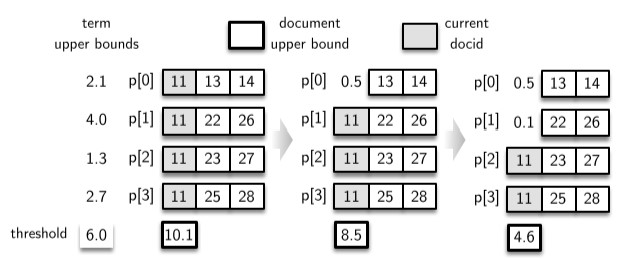
\includegraphics[scale = 1.8]{img/early termination.jpg}
        \label{early termination}
        \caption{Example of early termination}
\end{figure}

In the example, the current threshold value $\theta$ is 6.0, resulting from documents in the current top results. While scoring docID 11, the document upper bound is initially set to 10.1, the sum of the 4 term upper bounds. While postings are processed, the document upper bound is adjusted with the actual scores computed for each term. Hence, it decreases to 8.5 after the posting from the first posting list is processed. Since 8.5 > 6.0, we must continue to process the other posting lists. After the posting from the second list is processed, the document upper bound becomes 4.6. At this point we are sure that document 11 will never obtain a final score greater than 4.6 and since it is less than the current threshold, the postings of the last two lists can be ignored, and the processing of docID 11 can be terminated, proceeding to the
next docID.

\underline{\textbf{Dynamic pruning for DAAT}}

We now focus on some dynamic pruning algorithms for the DAAT strategy, \textbf{MaxScore} and \textbf{WAND}, which both maintain a term upper bound in the vocabulary for each posting list, which is used at runtime to take decisions on the early termination and/or skipping of certain postings/documents.

The \textbf{MaxScore} algorithm is a \textbf{safe up to $k$ strategy} aiming to boost the efficiency of the DAAT algorithm through the following observation. At some point during query processing, we can expect that the threshold will be large enough to prune documents appearing only in the posting list with the smallest term upper bound contribution. When this happens, the algorithm can \textbf{safely skip over documents} appearing only in that \textbf{posting list}, and can consider as top-$K$ candidate documents only those appearing in the remaining posting lists. Once a new candidate document must be fully scored, that posting list can be traversed in an AND mode to look for the candidate docID only. This observation can be applied to the remaining posting lists as the query processing proceeds and the threshold increases. 

A possible implementation is reported in Picture \ref{max score}.  

\begin{figure}[h!]
		\centering
		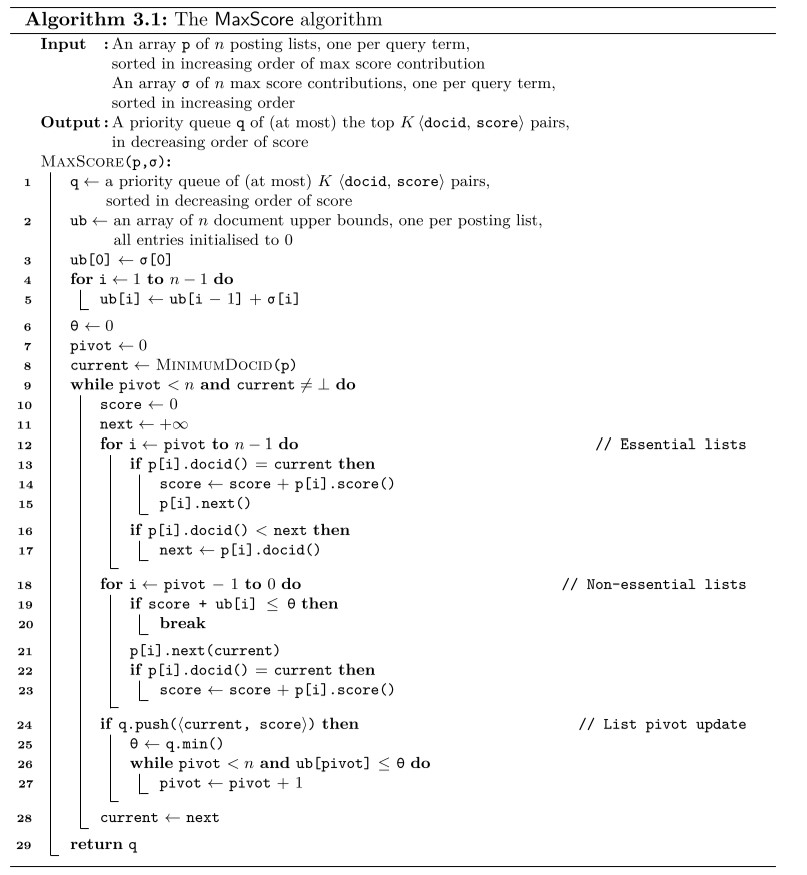
\includegraphics[scale = 1.4]{img/max score.jpg}
        \label{max score}
        \caption{Implementation of MaxScore algorithm}
\end{figure}

The algorithm takes as input two arrays of size $n$: the posting lists $p$ to be processed and the corresponding term upper bounds $\sigma$. Both arrays are sorted in increasing order of max score. At runtime, the posting lists are kept separated into two sub-lists by a pivot index, running from 0 to $n-1$. The posting lists indexed from the pivot up to $n$ form the \textit{essential lists}, while the remaining posting lists, if any, are the \textit{non-essential lists}. At any time during query processing, no document can be returned as a top-$K$ result if it only appears in the non-essential lists, i.e., at least one of the terms corresponding to the essential lists must occur in any top-$K$ document.

To update the pivot, we compute $n$ document upper bounds $ub$ (line 5). The entry $ub[0]$ contains the document upper bound for documents appearing just in $p[0]$, the entry $ub[1]$ contains the upper bound for documents appearing only in $p[0]$ and $p[1]$, and so on. While there is at least an essential list and there are documents to process (line 9), the MaxScore algorithm first processes the essential lists selecting the candidate docID as in DAAT, while storing the next docID to process (lines 12–17). Then, it proceeds by processing the non-essential lists by skipping to the candidate docID (lines 18-23). As soon as the pruning condition holds (line 19), we are sure that the candidate docID cannot be in the final top-$k$ documents, and the remaining posting lists can be skipped completely. If all the non-essential posting lists are processed, we check if the final score is high enough to enter.

Picture \ref{max score ex} shows the MaxScore pruning with 4 posting lists.

\begin{figure}[h!]
		\centering
		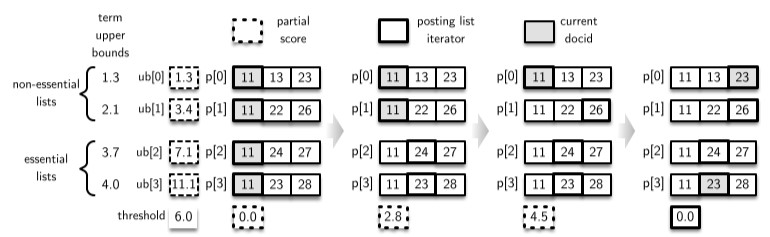
\includegraphics[scale = 1.8]{img/max score ex.jpg}
        \label{max score ex}
        \caption{Example of MaxScore algorithm}
\end{figure}

In the example, the current threshold value $\theta$ is 6.0, resulting from documents in the current top results. The posting lists are sorted by increasing term upper bound, and we have used the term upper bounds to compute the values of the array $ub$. Since $ub[1] = 3.4$ and $ub[2] = 7.1$, the pivot is set to 2, $p[0]$ and $p[1]$ are the \textit{non-essential lists}, while $p[2]$ and $p[3]$ are the \textit{essential lists}. We are processing the document with docID 11. Firstly, we process the \textit{essential lists} and compute the partial score of the document, keeping track of the next docID to process while advancing the posting list iterator of these lists by one step. Since, given the partial score computed so far, it is possible that docID 11 could exceed the current threshold (e.g., $2.8 + ub[1] = 2.8 + 3.4 = 6.2 > 6.0 = \theta$), we start processing the \textit{non-essential lists} for that document. After we process $p[1]$, skipping directly to the next docID greater than or equal to the next docID to process (e.g., 23), we get an updated partial score of 4.5. Now, since $ub[0]= 1.3$, we can safely ignore the first posting list (e.g., $4.5 + 1.3 = 5.8 < 6.0$), and skip directly to docID 23 using the $p.next(d)$ operator. Note that in the example we do not include the priority queue and pivot updates for simplicity.

The other algorithm is \textbf{WAND}. This algorithm is based on the \textit{WAND}, or \textit{Weak AND} operator, which takes as input a list of $n$ boolean variables $X_0, . . . ,X_{n−1}$, a list of $n$ associated weights $w_0, . . . , w_{n−1}$ and a threshold $\theta$. By definition, \textit{WAND} $(X_0, w_0, . . . ,X_{n−1}, w_{n−1}, \theta)$ is true if and only if: 

$$
\sum_{i = 0}^{n-1} w_ix_i \geq \theta
$$
, where $x_i$ is equal to 1 if $X_i$ is true, and 0 otherwise. Note that, with unary weights and a threshold equal to $n$ or 1, the \textit{WAND} operator implements the boolean \textit{AND} or \textit{OR}, respectively. 

Given a query $q = \{t_0, . . . , t_{n−1}\}$ and a document $d$, we can apply the \textit{WAND} operator in the following way. We assume that $X_i$ is true if and only if the term $t_i$ appears in document $d$, and we take the term upper bound $\sigma_{t_i} (d)$ as weight $w_i$. The threshold $\theta$ has the usual meaning, i.e., the smallest score among the top $K$ documents scored thus far during query processing. Hence the condition \textit{WAND} $(X_0, \sigma_{t_0}(d), . . . ,X_{n−1}, \sigma_{t_{n−1}}(d), \theta)$ evaluates to true if and only if:

$$
\sum_{i = 0}^{n-1}\sigma_{t_i}(d) \geq 0
$$

Assuming that all terms $t$ appear in document $d$, this inequality corresponds to the pruning condition $\sigma_d(q) \leq \theta $.

This algorithm exploits the \textit{WAND} operator to prune the documents whose \textit{WAND} evaluation is false, and then perform a full evaluation to compute the actual scores. Picture \ref{wand} represents a possible implementation of the algorithm.

\begin{figure}[h!]
		\centering
		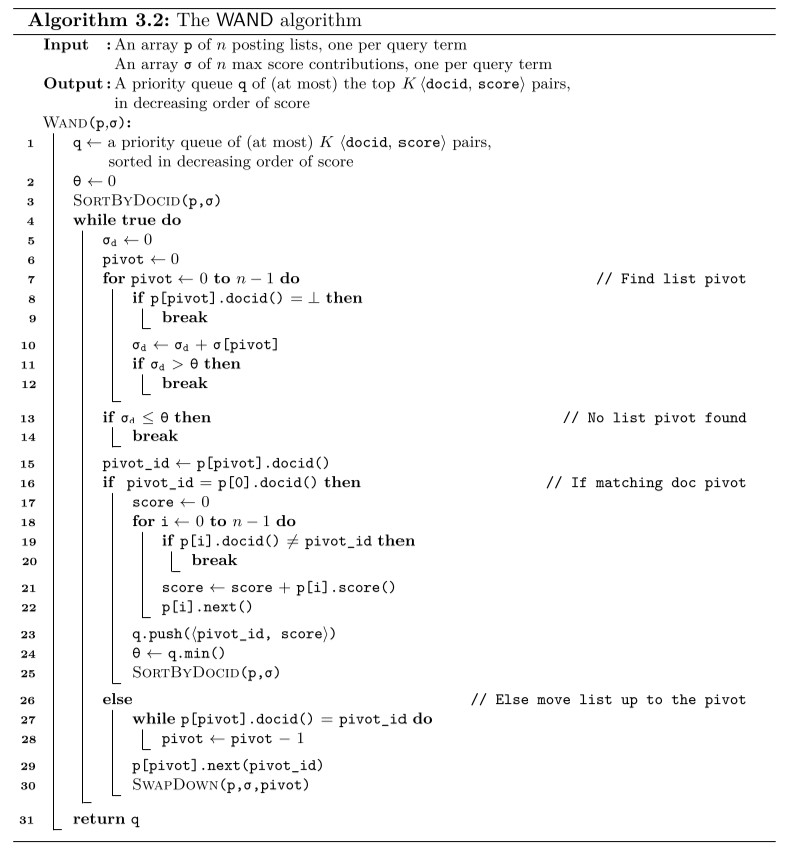
\includegraphics[scale = 1.8]{img/wand.jpg}
        \label{wand}
        \caption{WAND algorithm}
\end{figure}

\begin{itemize}
    \item INPUT: two arrays of size $n$: the posting lists $p$ to be processed and the corresponding term upper bounds $\sigma$. Note that they are not required to be sorted since they will be kept sorted though increasing the docIDs by the algorithm itself (lines 3 and 25). Indeed, the \textit{SortByDocid}$(p,\sigma)$ procedure guarantees that the array of posting lists are sorted by increasing docID and that the term upper bound $\sigma[i]$ always corresponds to the posting list $p[i]$;
    \item The core idea of the algorithm is to evaluate the \textit{WAND} operator (i.e., the pruning condition) one posting list at a time, accumulating the score of the candidate document in $\sigma_d$ (line 10);
    \item As soon as this value exceeds the current threshold (line 11), we have potentially identified a pivot docID (pivot\_id) that could enter the top $K$ documents. The pivot docID undergoes a full evaluation (lines 17–22) and might be included in the current top $K$ results (lines 23–24) only if it is present in all posting lists up to, and including, the list containing the pivot docID. Since the posting lists are sorted by docID, it is sufficient to test the pivot docID with the current posting’s docID of the first list p[0] (line 16);
    \item Otherwise, since the posting lists are sorted by docID, we can safely affirm that the pivot docID is the smallest docID among all posting lists from 0 to pivot that could enter the top $K$ results. The docID smaller than pivot\_id will never be able to accumulate enough term upper bounds to have a chance to beat the current threshold;
    \item Unfortunately, we cannot be sure that pivot\_id will be a candidate, since we do not know yet in which posting lists it appears. Thus, we “backtrack” to the first posting list whose iterator is not on the pivot docID (lines 27–28), and we move its iterator to the pivot\_id (or further) (line 29) using the p.next(d) operator. The \textit{SwapDown}$(p,\sigma,\textit{pivot})$ procedure on line 30 restores the docID-sorting of the posting lists by moving the pivot posting list and the associated term upper bound “down” to the correct position. Using the $p.\text{next}(d)$ operator means that skipping occurs, and hence the reading and decompression of skipped postings can be avoided;
    \item To conclude, note that if no pivot docID can be found (line 13), we are sure that no new document can beat the current threshold, and hence the algorithm can safely terminate.
\end{itemize}

Picture \ref{wand ex} illustrates a few \textit{WAND} iterations with 4 posting lists. In the example, the current threshold value $\theta$ is 6.0, resulting from documents in the current top results. 

\begin{figure}[h!]
		\centering
		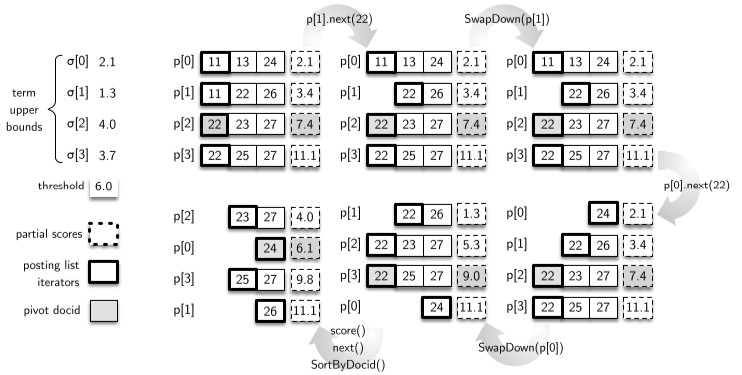
\includegraphics[scale = 1.8]{img/WAND example.jpg}
        \label{wand ex}
        \caption{Example of WAND algorithm}
\end{figure}

The posting list iterators are sorted by current docID. The next pivot id is 22 since neither 2.1 nor $2.1 + 1.3 = 3.4$ are greater than the current threshold, while $2.1 + 1.3 + 4.0 = 7.4$ does exceed the threshold. Since the $p[0]$ iterator is not 22, the only knowledge we have so far is that no docID smaller than 22 will have a score greater than the current threshold. Hence, we select $p[1]$ and we advance its iterator to 22, with no reordering of the posting lists since they are already sorted by docID. At the next iteration, our pivot docID is again 22, but we cannot fully score it since we do not know if $p[0]$ will actually contribute to the approximate score of the pivot docID, i.e., we do not know if $p[0]$ contains docID 22. We try to advance the $p[0]$ iterator to 22, but it skips to docID 24, forcing the move of $p[0]$ to the end of the array of iterators. At the next iteration, we are again considering docID 22: its approximate score now is 1.3 + 4.0 + 3.7 = 9.0, enough for a full processing, and since all posting lists up to the pivot docID include it, docID 22 undergoes a full evaluation, and a potential threshold update. During the full evaluation, the iterators of the involved posting lists are advanced to the next docID (line 22), hence a full reordering of the four lists is mandatory, to correctly select the next pivot docID (that, with the current threshold $\theta = 6.0$, will be 24, since $\sigma[2] + \sigma[0] = 4.0 + 2.1 = 6.1 > \theta)$.

Note that the \textit{WAND} optimisation is \textbf{safe up to $K$}, since the pruning condition is used to select the candidate docIDs. Nevertheless, aggressive (i.e., approximate) versions of \textit{WAND} have been proposed forcing the new candidate documents to beat the current threshold by a larger quantity.

\subsection{MIPS algorithms for dense vectors}\label{mips for dense}
We now focus on the solving methods for the MIPS problem when the documents and the queries are \textbf{dense vectors}, i.e., vectors characterized by very few zero entries. 

First of all, we try to reason about some of the techniques we used for sparse vectors, for example inverted indexes: are the suitable for dense vectors? The answer is no, since we recall that the objective of the inverted index data structure is to skip the dot product evaluation in presence of 0 entries. In this sense, the resulting data structure would be a very long list, which is inefficient. Moreover, we also cannot exploit the dynamic pruning algorithm, since the inverted lists are full of elements.

For these reasons, we have to consider new methods for speeding up the computation of the solution of MIPS problem in presence of dense vectors.

\subsubsection{Quantization methods}
In general, some documents of a collection can be very similar to each other (this is true from the nature of data), so the idea of \textbf{quantization methods} is to reduce the complexity of the problem by quantizing very similar documents, which are represented as points in a high-dimensional space, and then solve the MIPS problem considering only the representatives for each quantized region. From a mathematical point of view, we can define a codebook $C = \{ c_1, c_2, .., c_m \}$, with $c_i \in \mathbb{R}^n$, and a map $\pi : D \to [m]$. Then, the approximate solution of the MIPS problem is given by all the documents in $c_k$, where:

$$
c_k = \text{arg}\max_{c_{\pi(d)}} \langle c_{\pi(d)}, q \rangle
$$

, i.e. the documents contained in the quantized region which has a maximum inner product with the query. A visual representation of this method is provided in Picture \ref{quantization}.

\begin{figure}[h!]
		\centering
		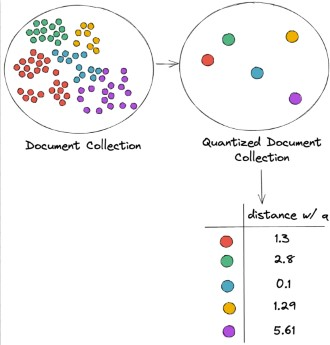
\includegraphics[scale = 1.8]{img/quantization.jpg}
        \label{quantization}
        \caption{Example of quantization}
\end{figure}

Finally, we can compare the approximate solution with the exact one by computing the \textit{recall} between the two sets of top-$k$.

An important \textbf{issue} about this methods relies in the so-called \textbf{curse of dimensionality}, a phenomenon for which, when the dimensionality of the vectors goes to $\infty$, the concepts of similarity and distance do not hold anymore.

For this reason, another idea that exploits quantization is called \textbf{product quantization}, and it works as follows: since the dot product is linear, we can rewrite is as:

$$
\langle q,d \rangle = \sum_{i = 1}^n q_i d_i = \sum_{i = 1}^n \sum_{j = 1}^n q_{ij} d_{ij} = \langle q_1, d_1 \rangle + \langle q_2, d_2 \rangle + .. + \langle q_1, d_1 \rangle = \sum_{i = 1}^M \langle q^{(i)},d^{(i)} \rangle
$$

, where $d^{(i)} \in \mathbb{R}^{n/M}$. In this sense, the idea is to break up both the vectors $q$ and $d$ into $M$ subvectors, each of which containing a quantized region of points called $C_i$. Then, for each $i$, we can compute the distance between $q^{(i)}$ and each of the points in $d^{(i)}$, in order to select the \textbf{representative} for each region, i.e. the point with minimum distance. Finally, we compute the dot product between $q^{(i)}$ and each representative $C_i$ and we sum up the scores, in order to get an approximate solution for the dot product between $q$ and $d$. A visual representation of this method is provided in Picture \ref{quantization2}. 

\begin{figure}[h!]
		\centering
		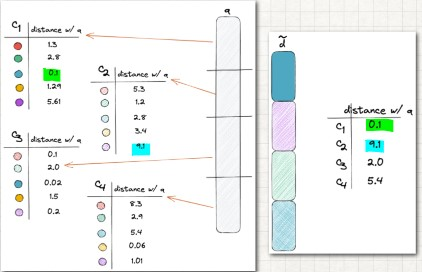
\includegraphics[scale = 2.0]{img/quantization_2.jpg}
        \label{quantization2}
        \caption{Example of product quantization}
\end{figure}

One \textbf{advantage} of this new method is that it is \textbf{efficient} in time, since the only operations that are involved are the \textbf{lookup} in the tables containing the distance between each segment of the query and all the points in a segment of the doc and the \textbf{summation} of the partial dot product scores. Moreover, this algorithm obtains \textbf{perfect results} if each segment contains a number of centroids which is equal to the number of points. On the other hand, this method is \textbf{useless} if we have one cluster per segment, and it is still heavy from a space point of view. 

For this reason, one last quantization method can be used, called \textbf{IVFPQ}, which works as follows: we cluster the collection of documents $D$ and we create an inverted index that maps cluster centers to list of points in that partition. Then, within each cluster we can apply \textit{product quantization} to the residuals $d - u$, where $u$ is the center of the cluster. A visual representation of this method is provided in Picture \ref{quantization3}.

\begin{figure}[h!]
		\centering
		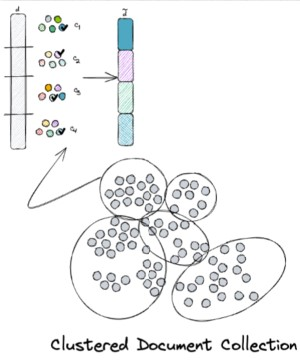
\includegraphics[scale = 2.0]{img/ivfpq.jpg}
        \label{quantization3}
        \caption{Example of IVFPQ}
\end{figure}

Finally, Picture \ref{quantization4} provides a comparison between the complexity, both in time and space, of quantization and product quantization methods.

\begin{figure}[h!]
		\centering
		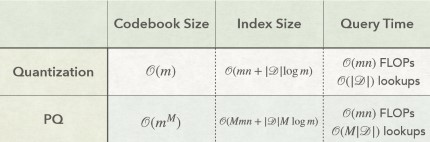
\includegraphics[scale = 2.0]{img/quantization_3.jpg}
        \label{quantization4}
        \caption{Comparison of quantization and product quantization}
\end{figure}

\subsubsection{Clustering methods}
Another important method is \textbf{clustering}, which works as follows:

\begin{enumerate}
    \item Cluster the documents into $m$ clusters with centroids $C = \{ c_1, c_2, .., c_m  \}$, with $c_i \in \mathbb{R}^n$
    \item Given a query $q$:
    \begin{enumerate}
        \item Compute the distance between the query and each of the centroid: $\langle c_i, q \rangle$
        \item Solve MIPS over the "closest" clusters.
    \end{enumerate}
\end{enumerate}

A visual representation is provided in Picture \ref{clustering}.

\begin{figure}[h!]
		\centering
		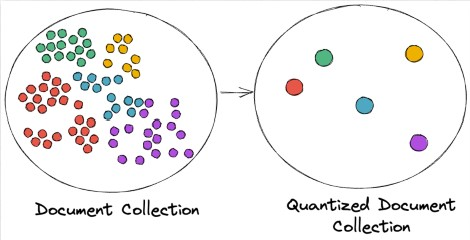
\includegraphics[scale = 2.0]{img/clustering.jpg}
        \label{clustering}
        \caption{Clustering method}
\end{figure}

Notice that this method is quite useful and effective when we can exploit distributed that are able to solve MIPS.

\subsubsection{Graph methods}
We now discuss the \textbf{graph methods}. 

Given two points $A$ and $B$, and a query point $q$, we can draw the line that is orthogonal to the line connecting $A$ and $B$, and divide the space into two regions:

$$
H_1 = \{ p | d(p,A) < d(p,B) \}
$$

$$
H_2 = \{ p | d(p,A) \geq d(p,B) \}
$$

, where $d(x,y) = ||x-y||_2$.

\begin{figure}[h!]
		\centering
		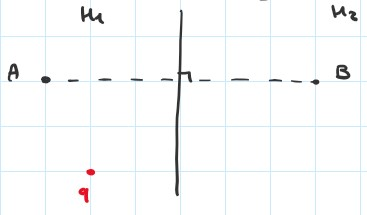
\includegraphics[scale = 1.6]{img/voronoi 1.jpg}
        \label{voronoi1}
        %\caption{Clustering method}
\end{figure}

If we have 3 points, the situation is the following one:

\begin{figure}[h!]
		\centering
		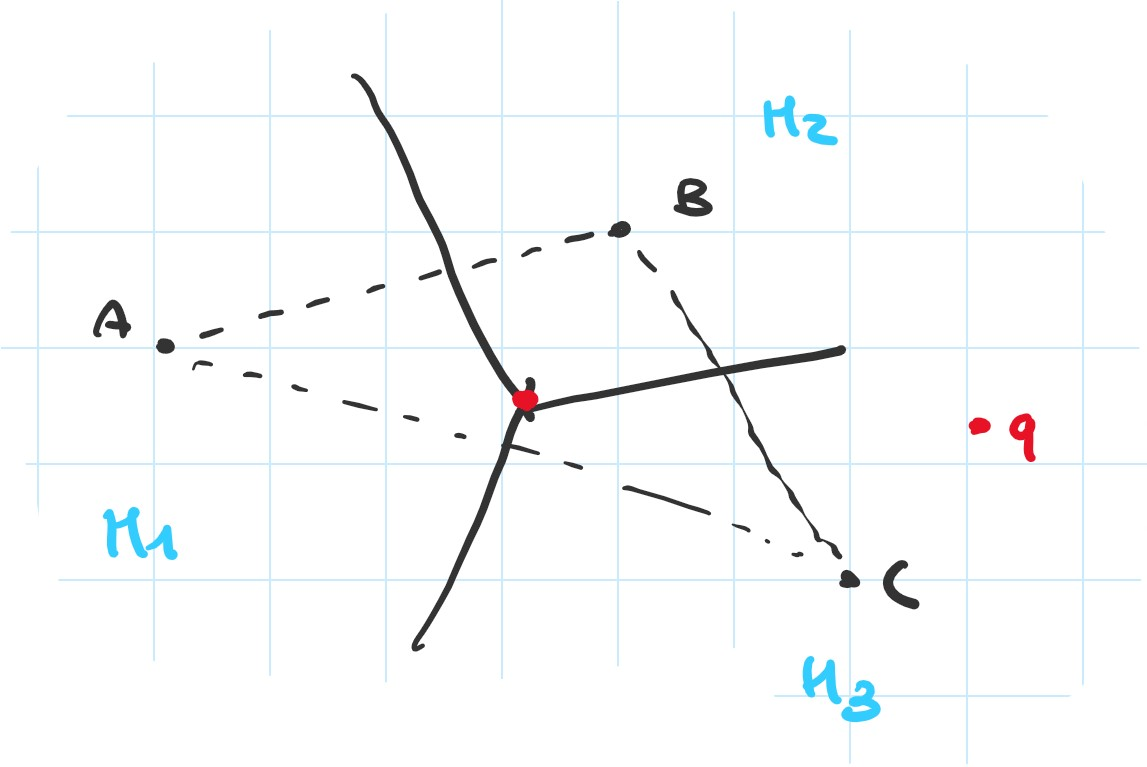
\includegraphics[scale = 0.6]{img/voronoi 2.jpg}
        \label{voronoi2}
        %\caption{Clustering method}
\end{figure}

Each of the $H_i$ is called \textbf{Voronoi region}, and they are formally defined as convex regions formed by the intersection of hyperplanes. A \textbf{Voronoi diagram} divides the space into $D$ Voronoi regions s.t. each point $d_i$ lies in exactly one Voronoi region. 

\begin{figure}[h!]
		\centering
		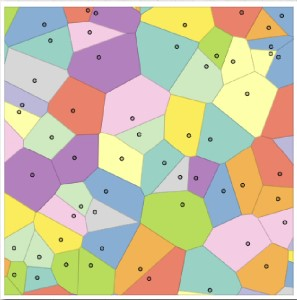
\includegraphics[scale = 1.8]{img/graph_1.jpg}
        \label{graph1}
        \caption{Voronoi diagram}
\end{figure}

Now we can introduce the \textbf{Delaunay graph}, which is a graph $G = (V,E)$ where $V = D$, i.e. the vertices are the documents, and $e_{ij} = 1 \iff H_i \cap H_j \neq \emptyset$.

\begin{figure}[h!]
		\centering
		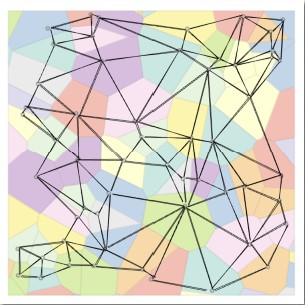
\includegraphics[scale = 1.8]{img/graph_2.jpg}
        \label{graph2}
        \caption{Delaunay graph}
\end{figure}

How can we exploit this graph to find the document point which is closest to a query point $q$? We can prove that a \textbf{greedy traversal} of the Delaunay graph guarantees the discovery of the \textbf{correct nearest neighbor} to a query point. However, in \textbf{high dimensions} the graph is almost \textbf{fully connected}, since the average degree in the Euclidean space grows exponentially in dimensions.

For this reason, we can approximate the Delaunay graph by considering a subgraph of the original one in which $e_{ij} = 1 \iff \forall d_k, d(d_i, d_j) \leq \text{max} \{ d(d_i, d_k), d(d_k, d_j) \}$. 

\begin{figure}[h!]
		\centering
		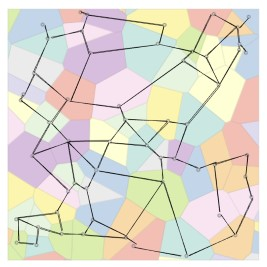
\includegraphics[scale = 1.8]{img/graph_3.jpg}
        \label{graph3}
        \caption{Approximation of the Delaunay graph}
\end{figure}
